%%
%% Copyright (c) 2018-2019 Weitian LI <liweitianux@sjtu.edu.cn>
%% Creative Commons BY 4.0
%%

\chapter{绪论}
\label{chap:introduction}

%=====================================================================
\section{研究背景}
\label{sec:background}

理解宇宙的结构、起源和演化,是人类孜孜不倦地追求的目标,在哲学和科学中占据重要地位。
经过无数人的努力,宇宙学的\ac{bbt}终于得以建立。
该理论已被大量观测证据所支持,比如星系的红移--距离关系(即 Hubble 定律)、
\ac{cmb}辐射、星系的大尺度分布、早期元素丰度、等等,
是目前宇宙学的标准模型。

根据大爆炸宇宙学模型,宇宙起源于约 138 亿年前的一次大爆炸,然后随着宇宙的膨胀,
温度以及能量密度都逐渐降低,宇宙主要经历了\ac{inflation}、\ac{bbn}、
\ac{recomb}、\ac{da}、形成第一代天体、\ac{reion}、形成星系及大尺度结构
等阶段,如\autoref{fig:univ-history} 所示。

\begin{figure}[!htp]
  \centering
  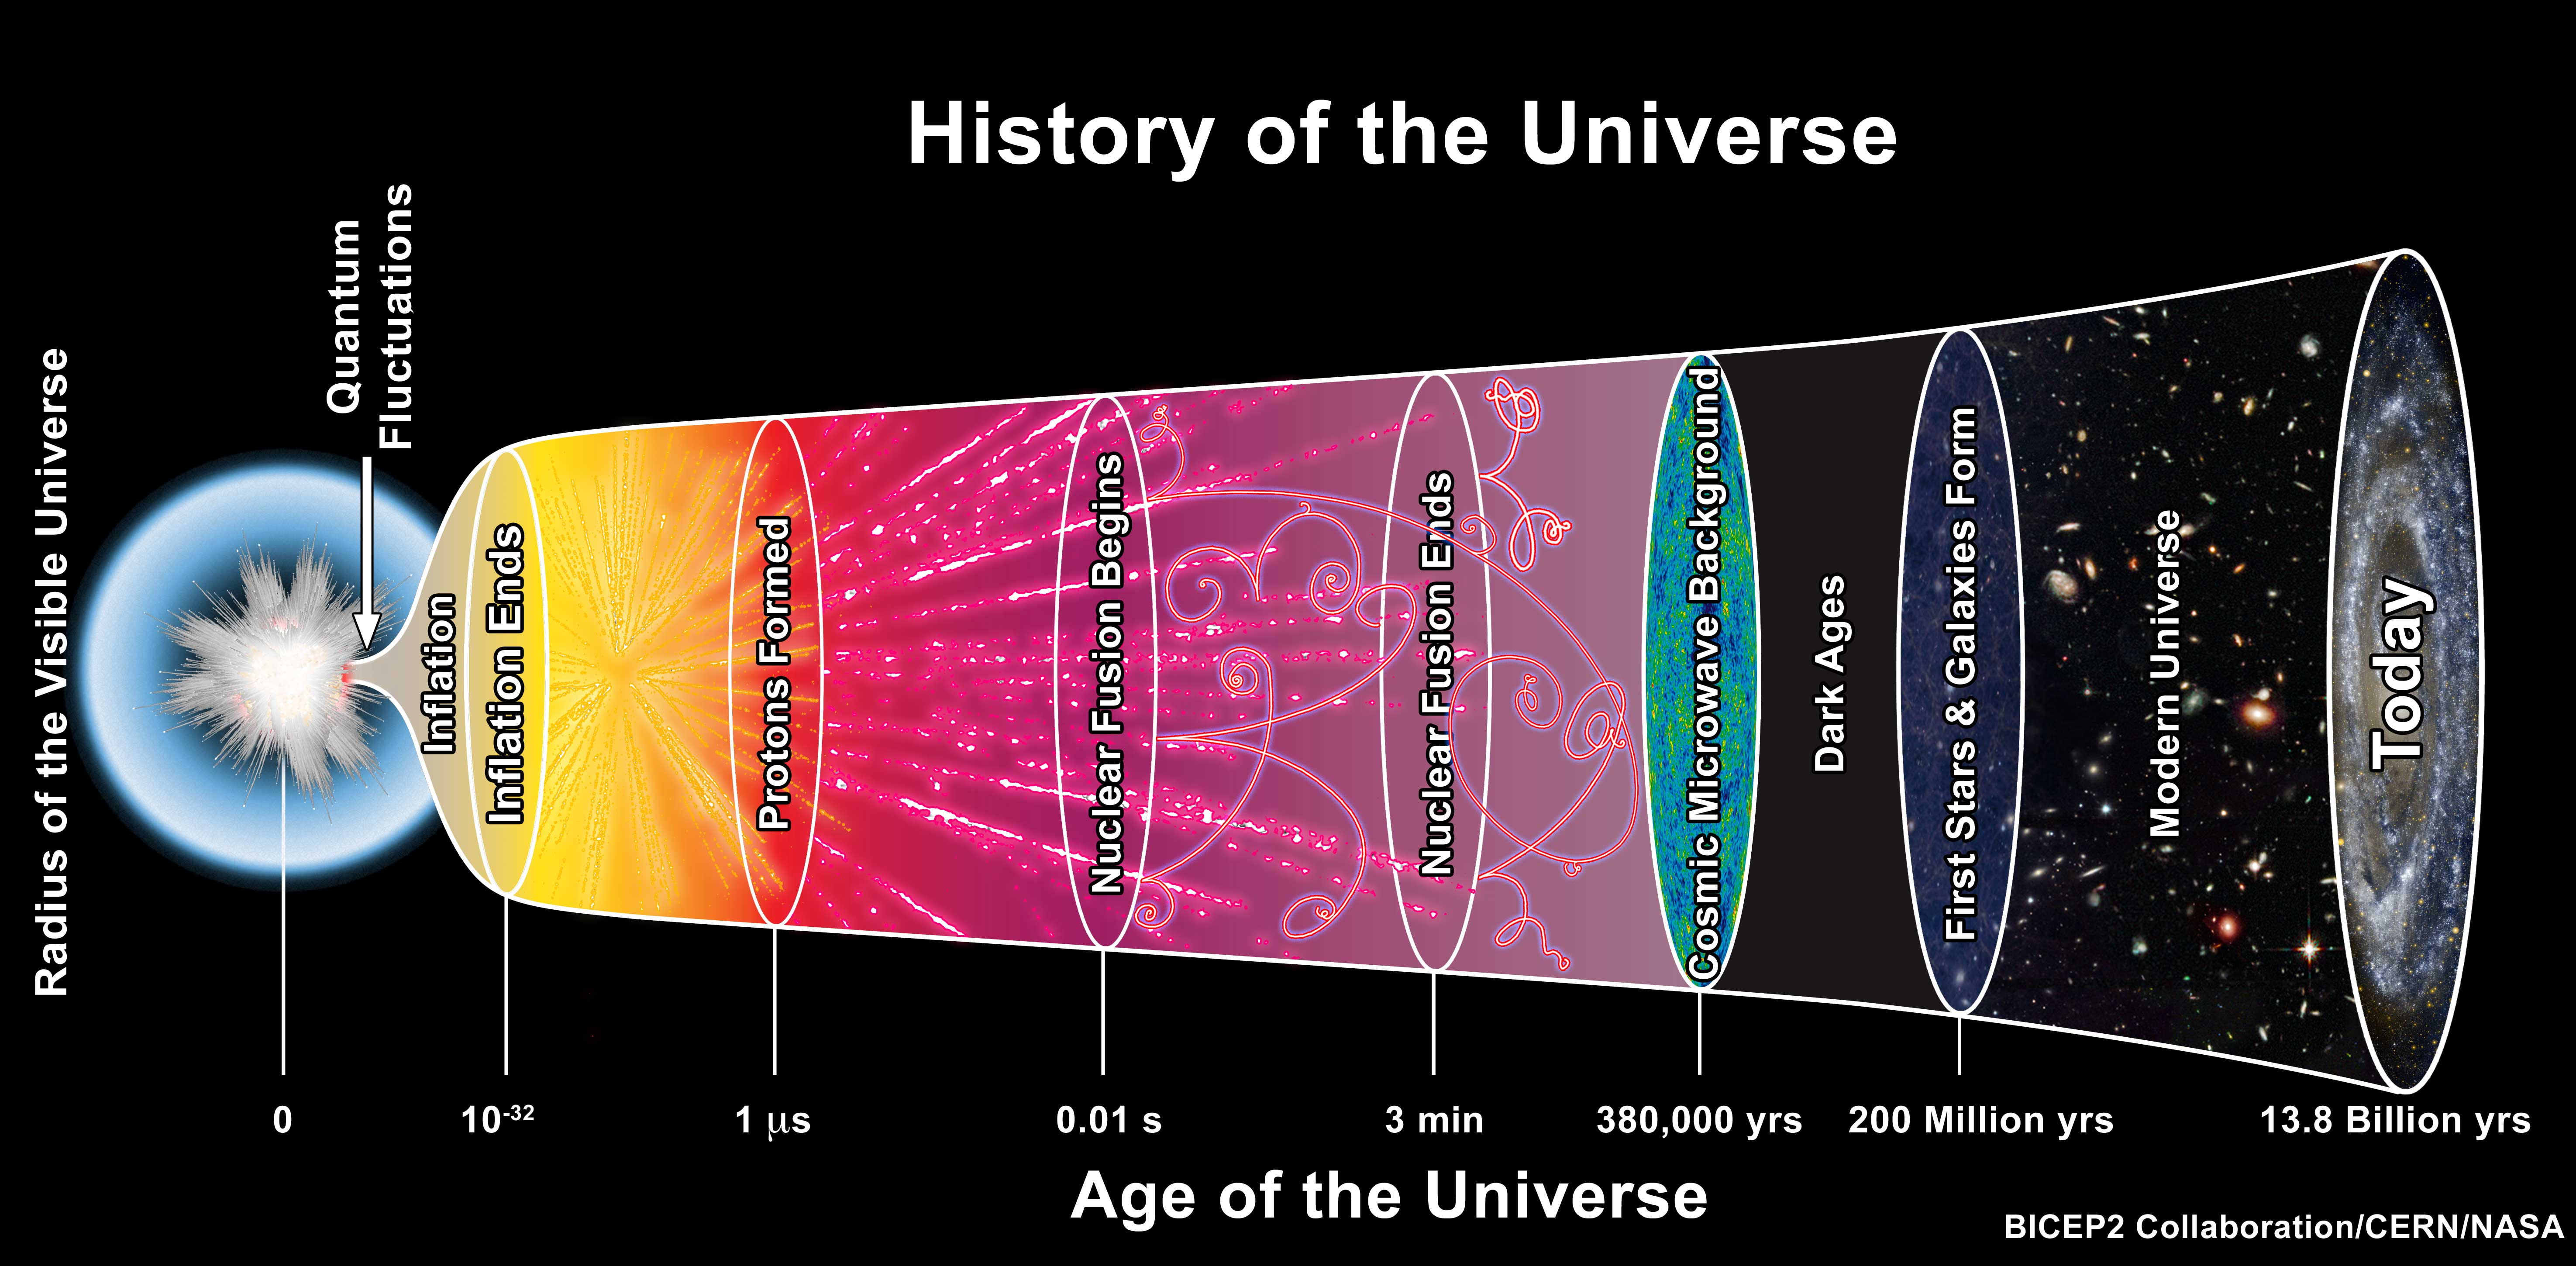
\includegraphics[width=\textwidth]{universe-history}
  \bicaption[宇宙的演化历史]{%
    宇宙从大爆炸到今天的演化历史。
  }{%
    The evolution of the Universe from the Big Bang
    to the present.
    \\\textcopyright{}
    \acuse{bicep,cern,nasa}
    \acs{bicep}2/\acs{cern}/\acs{nasa}; CC0 1.0.
  }
  \label{fig:univ-history}
\end{figure}

大爆炸之后约 40 万年,宇宙已冷却至大约 \SI{3000}{\kelvin},
于是自由电子被结合到中性原子之中,与重子物质脱耦的光子开始在宇宙中自由传播,
形成弥漫于整个宇宙的背景辐射,即今天所探测到的 \ac{cmb} 辐射。
但是,此时尚未形成发光的天体,因此宇宙进入了\acl{da}。
随着物质的密度扰动在引力作用下增长,第一代天体开始形成并产生辐射,使得重子物质
再次被逐步电离,宇宙从此结束\acl{da}并走入\ac{eor}。
随着各尺度上的天体结构的逐步形成与演化,重子物质被充分电离,宇宙也演化形成今天的格局。

\begin{figure}[!htp]
  \centering
  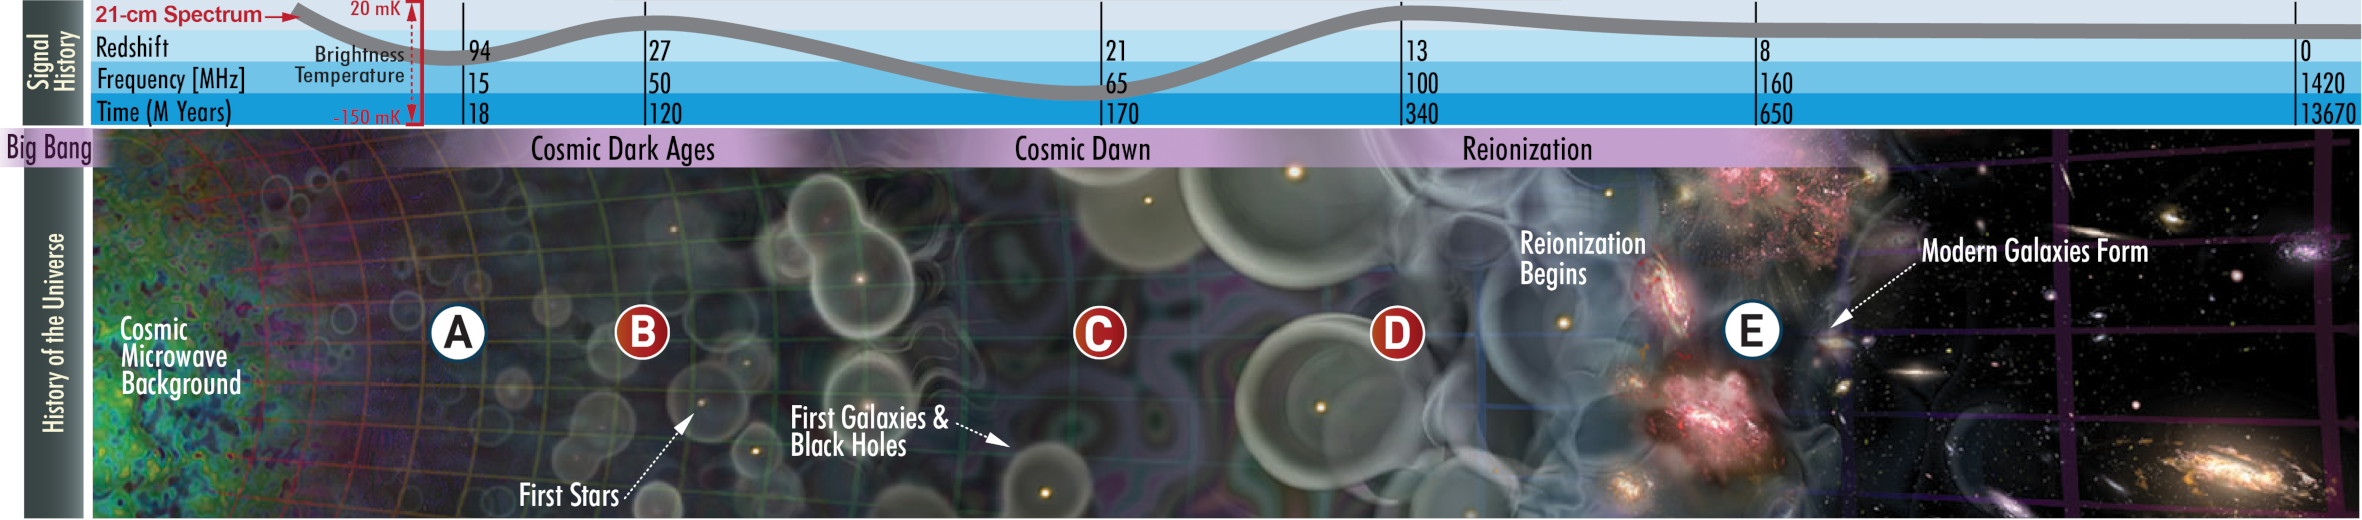
\includegraphics[width=\textwidth]{cosmic-stages-dare}
  \bicaption[宇宙的黑暗时期与再电离时期示意图]{%
    宇宙的\acl{da}与\acl{eor}示意图,其中显示了\acl{aoi} (A)、\acl{da} (B)、
    \acl{cd} (C) 以及\acl{eor} (D, E)。
    上方的粗曲线显示了理论预测的 \hisignal/的强度。
  }{%
    A schematic showing the \acs{da} and the \acs{eor}
    of the Universe, mainly including the \acs{aoi} (A),
    the \acs{da} (B), the \acs{cd} (C), and the \acs{eor} (D, E).
    The thick curve in the top panel shows the predicted intensity
    of the 21\,cm signal.
    \\\textcopyright{}
    \acuse{dare}\ac{dare},
    \url{http://lunar.colorado.edu/dare/science.html}, (2018-09-23).
  }
  \label{fig:cosmic-stages}
\end{figure}

我们已借助多波段观测掌握了大量有关宇宙近期演化
($\acs{z} \lesssim 6$;宇宙已充分电离之后)的信息;
通过研究 \ac{cmb},我们对宇宙的早期历史
($z \gtrsim 1100$;自由电子\acl{recomb}之前)有了深刻理解。
然而,我们对中间的那段时期($z \sim \numrange{6}{1100}$)却知之甚少。
这段时期可细分为以下四个阶段\cite{koopmans2015}:
\acl{aoi} (\acs{aoi}; $z \sim \numrange{200}{1100}$)、
\acl{da} ($z \sim \numrange{30}{200}$)、
\acl{cd} (\acs{cd}; $z \sim \numrange{15}{30}$)
以及\acl{eor} ($z \sim \numrange{6}{15}$),
如\autoref{fig:cosmic-stages} 所示。
对于其中距离我们相对较近的\acl{eor},
我们目前仅获得非常有限的间接观测信息,比如:
该时期的\ac{hi}对高红移类星体的 Ly$\alpha$ 吸收 \cite{becker2001}、
该时期的自由电子对 \ac{cmb} 光子的 Thomson 散射 \cite{kaplinghat2003}。
但是,我们仍然缺乏来自\acl{eor}的直接观测证据,
对该时期的基本性质和关键物理过程仍不清楚,比如:
第一代天体是何时以及如何形成的?
主要的电离源有哪些以及它们是如何影响再电离过程的?
电离氢区的尺度以及演化过程如何?
研究\acl{eor}的对于理解宇宙早期结构形成以及星系的形成与演化有重要意义,
是建立完整的宇宙演化图景的关键环节之一。
具体请参见 \citeay{fan2006}, \citeay{morales2010},
\citeay{pritchard2012}, \citeay{zaroubi2013},
\citeay{koopmans2015} 等综述文。

在\acl{eor}及其之前的\acl{da},尽管缺乏发光天体可供观测,
但是宇宙中丰富的\acl{hi}所辐射的 21\,cm 谱线
(以下简称 \emph{\hisignal/};
详见 \autoref{sec:21cm-signal})为探测该时期提供了有效途径。
对 \hisignal/的探测是目前对\acl{eor}及其之前的\acl{da}开展系统性
研究的最直接而有效的观测手段 \cite{koopmans2015,furlanetto2016}。

\acl{hi}的 21\,cm 谱线的本征频率约为 \SI{1420}{\MHz}。
源自\acl{eor}的 \hisignal/(以下简称 \emph{EoR 信号})经历显著红移后
应出现在约 \SIrange{90}{200}{\MHz},对应低频射电波段。
EoR 信号到达地球时已非常微弱,仅约几 \si{\mK} 至十几 \si{\mK},
因此需要具有极高灵敏度的低频观测设备才能捕获该信号。
目前的主流技术是采用大规模低频干涉阵列,已建成或正在建设的干涉阵列主要有:
\ac{21cma} \cite{zheng2016}、
\ac{gmrt} \cite{paciga2011}、
\ac{mwa} \cite{bowman2013,tingay2013}、
\ac{lofar} \cite{vanHaarlem2013}、
\ac{lwa} \cite{ellingson2009}、
\ac{paper} \cite{parsons2010}、
\ac{hera} \cite{deboer2017}、
\ac{ska} \cite{mellema2013,koopmans2015}。
然而,利用干涉阵列探测 EoR 信号仍面临诸多困难与挑战,其中主要包括:
识别并扣除强烈的前景干扰、扣除人工源的\ac{rfi}、修正电离层的扰动、
苛刻的仪器校准要求、海量数据处理和高动态范围成像。

在低频射电波段,强烈的前景干扰(主要源自银河系以及河外点源;
详见 \autoref{sec:fg-intro})比待探测的 EoR 信号高出约 5 个数量级;
即便按干涉阵列所测量的天空亮度涨落来衡量,前景干扰的涨落也是待测信号的数千倍
\cite{zaroubi2013}。
如何准确把握前景干扰并将其有效扣除,是成功探测 EoR 信号的关键。
由于低频射电观测和巡天数据的严重不足,我们对该波段的前景的了解非常有限,
无法达到探测 EoR 信号所要求的精度。
因此,我们需要挖掘已有海量的中高频射电观测以及其他多波段观测数据,
并结合逐渐增长的低频观测数据,深入理解低频射电前景辐射,构建并完善前景模型,
为识别并扣除前景干扰提供有力支撑。

虽然在本质上,前景辐射的频谱是光滑的,而 EoR 信号的频谱呈锯齿状,
两者具有很好的可区分性 \cite{wang2006,jelic2008,harker2009,wang2013}。
然而在实际情况中,受到干涉阵列的复杂仪器效应、观测干扰、数据处理技术的限制
等因素的影响,前景频谱的光滑性遭到破坏,导致 EoR 信号的提取变得尤其困难
\cite{liu2009ps,labropoulos2009,gehlot2018,mertens2018}。
如何研发出行之有效的前景处理和 EoR 信号提取算法,亦是当前的重要研究课题。


%=====================================================================
\section{研究内容}
\label{sec:content}

本文的研究内容分为以下两部分:
\begin{itemize}
\item
\emph{改进低频射电天空的模拟:}
深刻理解各前景成分的性质(如强度、空间分布、频谱结构)并充分把握它们对 EoR 探测
的干扰方式,是研发具有针对性的前景去除和 EoR 信号分离算法的前提与关键 (ref???)。
由于复杂的仪器效应和严重的观测干扰,低频干涉阵列的系统校准非常困难
\cite{noordam2004,intema2009,wijnholds2010,barry2016,gehlot2018},
严重制约仪器达到探测 EoR 信号所要求的极高灵敏度。
在现阶段缺乏足够可用的高质量低频射电观测数据的情况下,挖掘已有多波段观测数据并
准确模拟低频射电天空,是开展前景干扰研究以及 EoR 信号分离算法研发的可行办法。

\hspace{2\ccwd}%
在诸多前景成分之中,银河系的弥散辐射 [包括\ac{synrad}和\ac{brad}]
以及河外\ac{pntsrc}辐射是最主要的成分,目前已被广泛地研究和较好地理解
\cite{shaver1999,diMatteo2004,gleser2008,liu2012,murray2017,spinelli2018}。
除此之外,剩下的前景辐射主要来自河外\ac{extsrc},其中包括:
\ac{icm} \cite{feretti2012} 产生的\ac{rh}、\ac{rr}和\ac{rmh}、
\ac{gc}之外的\ac{igm} \cite{keshet2004}、
以及\ac{lsf} \cite{vazza2015}。
对于这些河外\acl{extsrc},已获得的观测证据不多,在低频射电波段更是不足。
关于它们将具体如何影响 EoR 探测,目前的理解非常有限,亟待深入且系统的研究。

\hspace{2\ccwd}%
与其他几类河外\acl{extsrc}相比,\acl{rh}拥有更多的观测证据和理论研究,支撑我们
构建一个更佳的模型用来模拟\acl{rh}的低频射电辐射,改进低频射电天空的模拟,
进而在考虑干涉阵列的实际仪器效应的情况下,有效地评估\acl{rh}对 EoR 探测的影响。

\item
\emph{研发 EoR 信号分离新算法:}
为了提取淹没于前景干扰中的 EoR 信号,一系列方法已被提出来用于处理前景
(详见 \autoref{sec:fg-methods})。
这些前景处理方法可大致分为\ac{fgrm}和\ac{fgavd}两大类,
但都依赖于一个重要前提:前景辐射的频谱必须非常光滑。
据此,这些方法通过构建一个模型来拟合光滑的前景成分并扣除,或者在功率谱空间尽量
避开前景污染区域,从而提取出微弱的 EoR 信号 \cite{chapman2016}。

\hspace{2\ccwd}%
然而在实际情况中,干涉阵列的\ac{beam}存在频率依赖效应(以下简称\emph{波束效应}),
即\acl{beam}的形状随观测频率而变化,因此 CLEAN 后残留的前景源会产生沿频率方向
快速变化的涨落,严重破坏前景频谱的光滑性 \cite{liu2009ps},
导致现有方法无法有效分辨前景干扰与 EoR 信号并分离出 EoR 信号
(详见 \autoref{sec:fdeffect})。

\hspace{2\ccwd}%
考虑到干涉列阵的\acl{beam}的形状非常复杂,为现有方法打造一个实际可用的模型
用以克服上述复杂的波束效应将很困难 \cite{lochner2015},
因此研发基于\ac{dl}的 EoR 信号分离新算法是一条更加可行且具有吸引力的途径
\cite{herbel2018,vafaeiSadr2019},
通过从数据中学习知识并自适应地优化模型,达到克服波束效应并分离 EoR 信号的目标。

\end{itemize}

本文的研究目标是:
(1)改进\acl{rh}的模拟,考虑干涉阵列的实际仪器效应,
获得更精细、更符合实际的低频射电天空的模拟图像,
进而有效地评估\acl{rh}对 EoR 探测的影响。
(2)研发基于\acl{dl}的能够有效克服干涉阵列的波束效应的 EoR 信号分离新算法,
并运用到上述模拟数据进行测试和优化。


%=====================================================================
\section{研究方案}
\label{sec:plan}

本文遵循以下主要步骤开展开展工作,完成研究内容,达到研究目标:
\begin{enumerate}
\item
调研\acl{rh}的相关理论研究和观测证据,理解其形成机制和演化规律,
构建模型并编程实现模拟\acl{rh}的低频射电辐射。
搜集\acl{rh}的现有观测数据,调节模型的参数,获得可靠的模拟结果。

\item
采用典型的干涉阵列(如 SKA1-Low)的布局方案,对上一步所得的\ac{skymap}
开展模拟观测,得到\ac{vis}数据,再利用 CLEAN 算法成像获得相应的“观测”图像。
通过这种\ac{e2e}模拟,干涉阵列的复杂仪器效应(如本文关注的波束效应)得以
有效地整合到研究流程之中。

\item
基于上述模拟所得的“观测”图像,利用一维和二维\ac{ps},对比\acl{rh}和
EoR 信号的异同,量化\acl{rh}在运用\acl{fgrm}或\acl{fgavd}的情况下
对 EoR 探测的影响,有效评估\acl{rh}作为前景干扰成分的重要程度。

\item
对比分析目前的主流\acl{dl}方法,筛选出合适的算法并加以必要的改进,
适用到此处的 EoR 信号分离场景。
利用已有模拟数据对算法进行训练和调优,挑选出满足要求的最佳算法。

\end{enumerate}


%=====================================================================
\section{本文框架}
\label{sec:structure}

本文余下章节安排如下:
\autoref{chap:interferometry}将介绍射电天文学和射电干涉技术的基础知识,
包括基本辐射理论、天线原理、干涉阵列及综合孔径成像等。
在\autoref{chap:detection},我们将介绍利用\acl{hi}
\hisignal/探测宇宙再电离时期的方法和困难、以及前景处理方法。
在\autoref{chap:simulation},我们首先模拟各前景成分和 EoR 信号的\acl{skymap},
然后进行干涉阵列的模拟观测,得到整合了实际仪器效应的观测图像。
据此,我们在\autoref{chap:halo}借助\acl{ps}量化评估\acl{rh}对
EoR 探测的具体影响。
\autoref{chap:cdae}将阐述我们提出的基于\acl{dl}的 EoR 分离新算法并演示其效果。
最后,我们对全文进行总结并简要展望。

全文采用一个由 \lcdm/ 模型描述的平直宇宙,具体参数为:
$\acs{H0} = 100\,\acs{h} = \SI{71}{\km\per\second\per\Mpc}$、
$\acs{Om0} = 0.27$、
$\acs{Ol0} = 1 - \acs{Om0} = 0.73$、
$\acs{Ob0} = 0.046$、
$\acs{ns} = 0.96$ 以及 $\acs{sigma8} = 0.81$。
如无额外说明,本文给出的误差对应 \SI{68}{\percent} 的置信水平;
使用的幂律谱形式为 $\acs{Sfreq} \propto \acs{freq}^{-\acs{Sidx}}$,
其中 \acs{Sfreq} 为\acl{Sfreq}、\acs{Sidx} 为\acl{Sidx}。
本文使用的中文术语遵循《英汉天文学名词数据库》
\footnote{英汉天文学名词数据库:\url{http://astrodict.china-vo.org/}}。


%% EOF
